\subsubsection{Fine-tuning on small clinical datasets}

We assessed the generalizability of our baseline model by fine-tuning it using small datasets from different institutions (including EPISURG), with different scanners, voxel resolution and acquisition protocols (\sectionref{sec:episurg,sec:multicenter}).
Additionally, we fine-tuned the model on 20 cases from EPISURG with the lowest \ac{DSC} (\sectionref{sec:self}).

For each dataset, we load the pretrained baseline model, initialize the optimizer with an initial learning rate of $5 \times 10^{-4}$, initialize the learning rate scheduler and fine-tune all layers simultaneously for 40 epochs using 5-fold cross-validation.
We use model weights from the epoch with the lowest mean validation loss for evaluation.
To minimize data leakage, we determined the above hyperparameters using the validation set of one fold in the \textit{Milan} dataset.

We observed a consistent increase in \ac{DSC} for all fine-tuned models, up to a maximum of 89.2 (13.3) for the \textit{Milan} dataset.
For comparison, inter-rater agreement between human annotators in our previous study was 84.0 (9.9) \cite{perez-garcia_simulation_2020}.
%Note that the labels in EPISURG used for training and evaluation were all generated by the same human rater.

Quantitative and qualitative evaluations are illustrated in \figureref{fig:finetuning_quant,fig:finetuning_qual}, respectively.

% \comment{
% \begin{table}
%     \centering
%     \caption{%
%         Results of finetuning the baseline model (trained with simulated resections only) on small datasets from different institutions using 5-fold cross validation.
%         Asterisks indicate statistical significance
%     }
%     \label{tab:finetune}
%     \begin{tabular}{lccl}
%         \toprule
%         \textbf{Dataset}    & \textbf{Subjects} & \textbf{SelfSL only} & \textbf{Finetuning} \\
%         \midrule
%         \textbf{Milan}      &                20 &             81.7 (16.4) &         89.2 (13.3)*   \\ % 33
%         \textbf{Paris}      &                19 &             82.4 (36.4) &         84.1 (19.8)    \\ % 40
%         \textbf{Strasbourg} &                33 &             74.9 (24.2) &         80.2 (20.1)    \\ % 36
%         \textbf{EPISURG} &                  133 &             80.5 (18.7) &         85.2 (10.8)*** \\ % 41
%         \textbf{EPISURG (worst)} &           20 &             19.2 (38.7) &         48.4 (51.4)*   \\ % 38
%         % \textbf{Glioma (KCL)} &              18 &             xx.x (xx.x) &         xx.x (xx.x) \\ %
%         \bottomrule
%     \end{tabular}
% \end{table}
% }


\begin{figure}
    \centering
    \floatconts
    {fig:finetuning_quant}
    {\caption{%
        \ac{DSC} without (blue) and with (orange) finetuning of the self-supervised model.
        Horizontal lines in the boxes represent the first, second (median) and third quartiles.
        Numbers in parentheses indicate subjects per dataset.
    }}
    {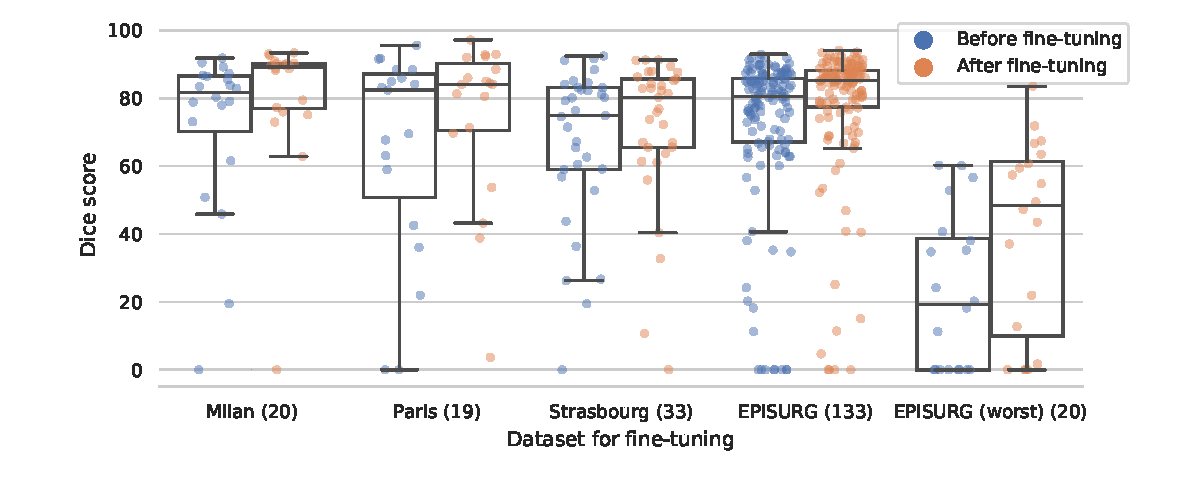
\includegraphics[width=\linewidth]{boxplot_finetuning}}
\end{figure}


\begin{figure}[ht!]
    \centering
    \floatconts
    {fig:finetuning_qual}
    {\caption{%
        Qualitative evaluation of fine-tuning for the \textit{Strasbourg} (left) and EPISURG (right) datasets.
        Rows correspond, from top to bottom, to cases for which the \ac{DSC}
        1) increased,
        2) remained high,
        3) remained low and
        4) decreased
        after fine-tuning the self-supervised model.
        Manual annotations (green) and model predictions (magenta) are overlaid.
    }}
    {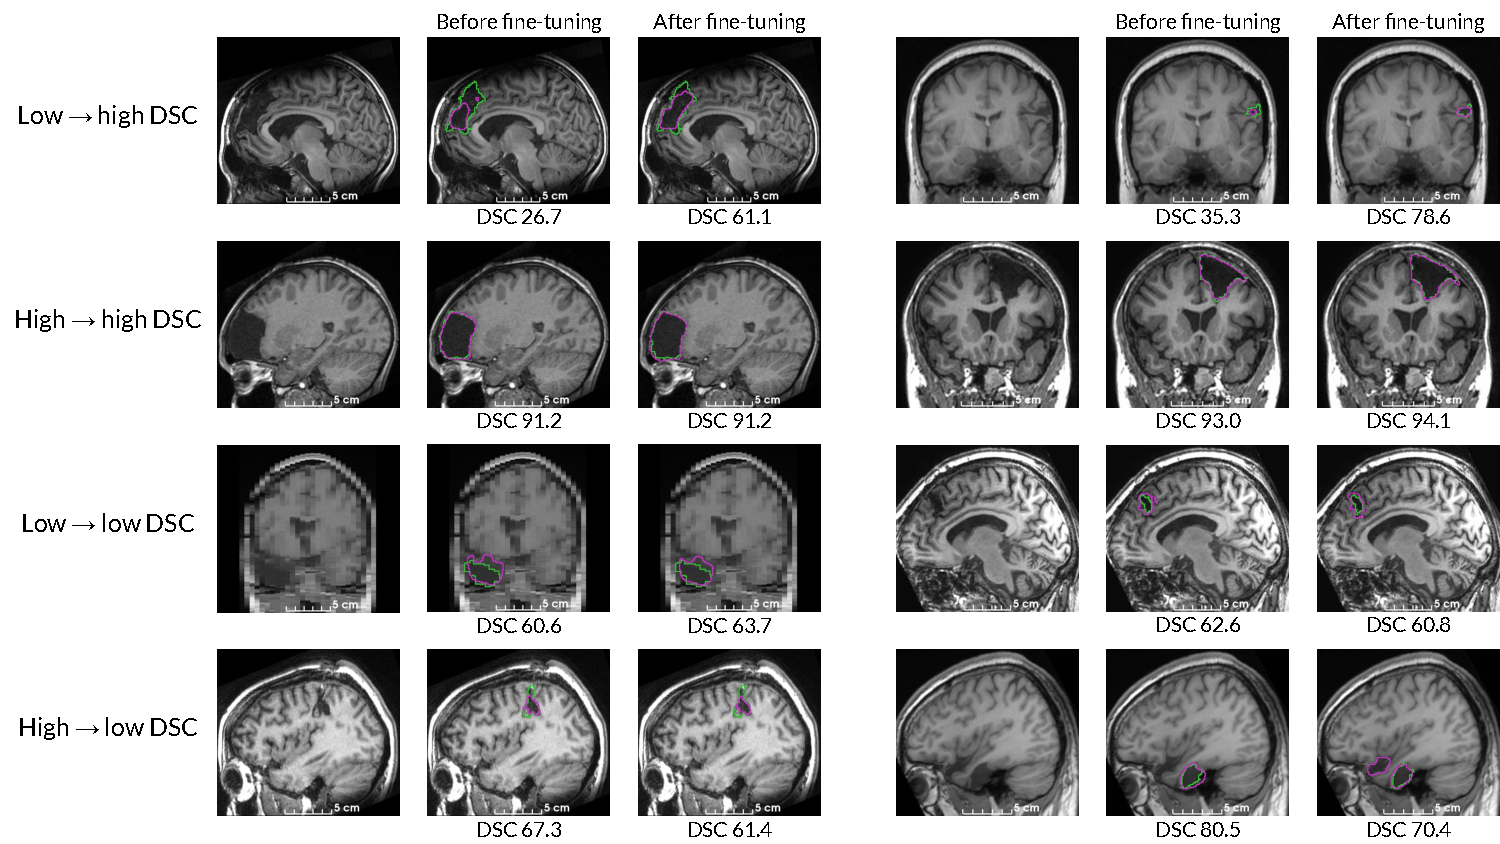
\includegraphics[width=\linewidth]{finetune}}
\end{figure}